 \documentclass[c]{beamer}
%\documentclass{beamer}
\listfiles

\mode<presentation>
{
  %\usetheme[deutsch,titlepage0]{KIT}
\usetheme[deutsch]{KIT}
% \usetheme{KIT}

%%  \usefonttheme{structurebold}

  \setbeamercovered{transparent}

  \setbeamertemplate{enumerate items}[circle]
  %\setbeamertemplate{enumerate items}[ball]

}
\usepackage{babel}
\date{}
%\DateText

\newlength{\Ku}
\setlength{\Ku}{1.43375pt}

\usepackage[utf8]{inputenc}
\usepackage[TS1,T1]{fontenc}
\usepackage{array}
\usepackage{multicol}
\usepackage{lipsum}
\usepackage[]{algorithm2e}
\usepackage{amsmath}
\usepackage{color}

\usenavigationsymbols
%\usenavigationsymbols[sfHhdb]
%\usenavigationsymbols[sfhHb]

\subtitle{Algorithmen I SS 14}
\author[]{Lena Winter}

\AuthorTitleSep{\relax}

\institute[ITI]{Institut für Theoretische Informatik}

\TitleImage[width=\titleimagewd]{images/title}

\newlength{\tmplen}

\newcommand{\verysmall}{\fontsize{6pt}{8.6pt}\selectfont}

\title[Algorithmen I SS 14]{Tutorium 4}

\usepackage{alltt}

\TitleImage[width=\titleimagewd]{images/title}

\definecolor{english}{rgb}{0.0, 0.5, 0.0}

\begin{document}

\begin{frame}
  \maketitle
\end{frame}


\begin{frame}
	\begin{center}
		\Huge
		Sortieren
	\end{center}
\end{frame}

\begin{frame}{Eigenschaften von Sortieralgorithmen}
	\begin{block}{in-place}
		Benötigt nur konstant viel Speicherplatz.
	\end{block}
	\begin{block}{stabil}
		Gleiche Elemente werden nicht vertauscht.

		$\langle 3, {\color{red}{2}}, 1, {\color{english}{2}}\rangle$ (unsortiert)\\
		$\langle 1, {\color{english}{2}}, {\color{red}{2}}, 3\rangle$ (nicht-stabil sortiert)\\
		$\langle 1, {\color{red}{2}}, {\color{english}{2}}, 3\rangle$ (stabil sortiert)
	\end{block}
\end{frame}

\begin{frame}
	\frametitle{Selectionsort}
	\begin{itemize}
		\item Funktionsweise:
		\begin{itemize}
			\item wähle immer das kleinste Element aus der Restmenge
		\end{itemize}
		\item Laufzeit: $\sum_{k=1}^{n-1} (n - k) = \sum_{k=1}^{n-1} k = \frac{n(n-1)}{2} \in \Theta(n^2)$
		\item {\color{english}inplace}
		\item {\color{english}stable}
	\end{itemize}
\end{frame}

\begin{frame}
	\frametitle{Insertionsort}
	\begin{itemize}
		\item Funktionsweise:
		\begin{itemize}
			\item nimm nächsten Wert und füge ihn an der passenden Stelle ein
		\end{itemize}
		\item Laufzeiten:
		\begin{itemize}
			\item Best Case: $\mathcal{O}(n)$ (bereits sortierte Folge)
			\item Average Case: $\mathcal{O}(n^2)$ (siehe Übung)
			\item Worst Case: $\mathcal{O}(n^2)$ (absteigend sortierte Folge)
		\end{itemize}
		\item {\color{english}inplace}
		\item {\color{english} stable}
	\end{itemize}
\end{frame}

\begin{frame}
	\frametitle{Mergesort}
	\begin{itemize}
		\item Funktionsweise:
		\begin{itemize}
			\item Divide and Conquer
			\item rekursives Aufteilen der Folge in jeweils zwei Subfolgen
			\item Mergen der sortierten Subfolgen bis nur noch eine Folge übrig bleibt
		\end{itemize}
		\item Laufzeit: $\mathcal{O}(n \log{n})$
		\item {\color{red} nicht inplace}
		\item {\color{english} stable}
	\end{itemize}
\end{frame}

\begin{frame}
	\frametitle{Quicksort}
	\begin{itemize}
		\item Funktionsweise:
		\begin{itemize}
			\item Teile Menge anhand eines Pivot-Elements in kleinere und größere Elemente, sortiere dann rekursiv weiter
		\end{itemize}
		\item Laufzeiten:
		\begin{itemize}
			\item Best Case: $\mathcal{O}(n \log{n})$
			\item Average Case: $\mathcal{O}(n \log{n})$
			\item Worst Case: $\mathcal{O}(n^2)$
		\end{itemize}
		\item {\color{red} nicht wirklich inplace} (nur "`inplace"')
		\item {\color{red} nicht stable}
	\end{itemize}
\end{frame}

\begin{frame}{Beispiel}
	Sortiere $\langle 58, 38, 97, 68, 6, 21, 37, 54, 24, 16, 65\rangle$

	\begin{enumerate}
		\item Selectionsort
		\item Insertionsort
		\item Mergesort
		\item Quicksort (Pivot: erstes Element)
	\end{enumerate}
\end{frame}

\begin{frame}{Kreativaufgabe}
	\begin{block}{Definition}
		\textbf{$p$-Perzentil}: Kleinstes Element einer Menge, für das $p \vert M \vert$ aller Elemente aus der Menge kleiner sind.
	\end{block}
	\begin{block}{Aufgabe}
		\begin{itemize}
			\item Gegeben:
				\begin{itemize}
					\item Array mit $n$ Elementen (unsortiert, vergleichbar)
					\item Medianfunktion: Berechne Median von einem Teilarray mit $m$ Elementen in $\mathcal{O}(m)$
				\end{itemize}
			\item Gesucht:
				\begin{enumerate}
					\item Finde einen Algorithmus, der das $\frac{1}{3}$-Perzentil in $\mathcal{O}(n)$ berechnet.
					\item Finde einen Algorithmus, der die $\frac{1}{3^{k-1}}, \frac{1}{3^{k-2}}, \dots, \frac{1}{3}$-Perzentile in $\mathcal{O}(n)$ (nicht in $\mathcal{O}(n k)$) berechnet.
					\item Beides geht inplace.
				\end{enumerate}
		\end{itemize}
	\end{block}
\end{frame}

\begin{frame}
	\frametitle{Ineffective Sorts}
	\begin{center}
		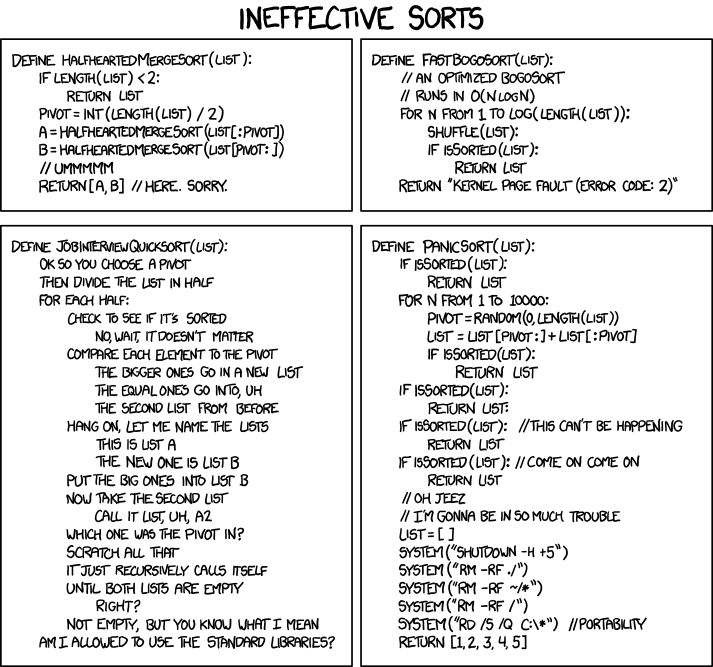
\includegraphics[width=\textwidth,height=\textheight,keepaspectratio]{images/ineffective_sorts}
	\end{center}
\end{frame}

\end{document}
